% Template for ICIP-2013 paper; to be used with:
%          spconf.sty  - ICASSP/ICIP LaTeX style file, and
%          IEEEbib.bst - IEEE bibliography style file.
% --------------------------------------------------------------------------
\documentclass{article}
\usepackage{spconf,amsmath,graphicx}
% 한글 패키지
\usepackage{kotex}
\usepackage[unicode, hidelinks]{hyperref}
\usepackage{subfigure}

% *** MATH PACKAGES ***
%
\DeclareMathOperator*{\argmin}{argmin}
\usepackage{amsfonts}

% Example definitions.
% --------------------
\def\x{{\mathbf x}}
\def\L{{\cal L}}

% Title.
% ------
\title{A Novel Filtering Approach for Robust and Fast Keypoint Matching in Mobile Environment}
%
% Single address.
% ---------------
\name{Jonghoon Seo, Seungho Chae,Yoonsik Yang, Heeseung Choi, Tack-Don Han \thanks{Thanks to KIST and NFS for funding.}}
\address{Author Affiliation(s)}
%
% For example:
% ------------
%\address{School\\
%	Department\\
%	Address}
%
% Two addresses (uncomment and modify for two-address case).
% ----------------------------------------------------------
%\twoauthors
%  {A. Author-one, B. Author-two\sthanks{Thanks to XYZ agency for funding.}}
%	{School A-B\\
%	Department A-B\\
%	Address A-B}
%  {C. Author-three, D. Author-four\sthanks{The fourth author performed the work
%	while at ...}}
%	{School C-D\\
%	Department C-D\\
%	Address C-D}
%
\begin{document}
%\ninept
%
\maketitle
%
\begin{abstract}
The abstract should appear at the top of the left-hand column of text, about
0.5 inch (12 mm) below the title area and no more than 3.125 inches (80 mm) in
length.  Leave a 0.5 inch (12 mm) space between the end of the abstract and the
beginning of the main text.  The abstract should contain about 100 to 150
words, and should be identical to the abstract text submitted electronically
along with the paper cover sheet.  All manuscripts must be in English, printed
in black ink.
\end{abstract}
%
\begin{keywords}
One, two, three, four, five
\end{keywords}
%
%!TEX root = ../icip_jseo.tex
% -*- root: ../icip_jseo.tex -*-

\section{Introduction}
\label{sec:intro}

Image matching is a fundamental problem in a variety of computer vision applications, including object recognition\cite{nister_scalable_2006}, panorama stitching\cite{brown_recognising_2003}, and augmented reality\cite{wagner_multiple_2009}. To accomplish image matching, keypoint-based local matching is widely used, since it can provide relatively high matching quality against severe occlusion and do not require segmentation for regions of interest. Also, recent work has concentrated on making invariant to image transformation with low computing power\cite{carrera_robust_2007,mikolajczyk_performance_2005}.

% To enhance the image matching quality in various environments, many related techniques have been proposed, such as keypoint-based local matching, histogram-based global matching\cite{le_improving_2013}, color-based matching\cite{mehtre_color_1995}, and template-based matching\cite{korman_fast-match:_2013}, etc. Among them, keypoint detection and matching has created great interest 

The overall flowchart of keypoint matching and recognition is shown in Fig. \ref{fig:on_offline_process}. This procedure can be divided into two main phases: offline learning (or training) and online testing procedure. Offline learning is a prerequisite to online matching process. In offline learning phase, a set of reference images to be recognized is analyzed and stored a set of descriptors in a database. In online testing phase, a newly captured image is analyzed and compared with the reference images in the database to find a nearest reference image. 
% In each phase, common procedures for matching are keypoint detection, description, and matching. To analyze training images, at first, keypoints are detected from the images. Then, from those keypoints, local textures are analyzed and described. In this procedure, to provide robustness against rotation, scale, perspective transform, descriptors are constructed. Then, to be used in online phase, efficient matching structures, as databases, are constructed, such as partitioning trees\cite{arya_optimal_1998,beis_shape_1997}, hashing\cite{salakhutdinov_semantic_2009,lv_multi-probe_2007}. In the online matching phase, the database is used to find the most similar corresponding keypoints pair with a given query image. To find the most similar keypoint pairs, with given a query image, keypoints are detected, detected keypoints are described about local texture, and compared with the preconstructed database.

\begin{figure}[hb!]
\centering
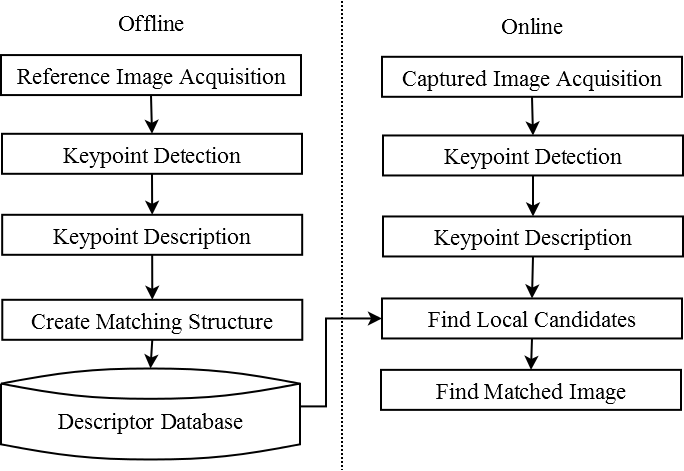
\includegraphics[width=1.0\columnwidth]{1_introduction/process}
\caption{Overall process of conventional keypoint-based matching}
\label{fig:on_offline_process}
\end{figure}

Conventional keypoint matching methods stores almost every keypoints which are detected by keypoint detection process. Keypoint detection processes are designed to extract repeatable keypoints and robust against arbitrary image transformation. Then, detected keypoints are independent to the follow matching procedures, and do not reflect quality of descriptors. Therefore, as seen Fig. \ref{fig:example_of_bad_features}, some keypoints are not distinguishable, and they tend to cause inter-keypoint confusion and miss matching. Also, those detected keypoints are stored in database and are compared with keypoints in query images in every frame while matching. Then, it decreases the speed of matching. To overcome these problem, in offline learning procedure, detected keypoints are evaluated with respect to proposed matching quality criteria and filtered by the goodness score. With this filtering method, only a small subset of keypoints is stored in the database. Accordingly, it provides more improved matching performance with faster matching speed.

\begin{figure}[ht!]
\centering

\includegraphics[width=0.5\columnwidth]{1_introduction/checkerboard}
\caption{Example of high repeatable but poor distinguishable keypoints. Conventional keypoint matching systems do not consider the discriminability of keypoints, so these keypoints usually stored and negatively affected matching.}
\label{fig:example_of_bad_features}
\end{figure}

Especially, mobile devices still have insufficient computing power and limited memory compared to desktop, so there is an urgent need of effective processing methods for image matching. However, conventional keypoint matching approaches stored redundant keypoints into database, and these redundant keypoints may are compared in every frame. So, matching speed will be decreased and this causes problem in the mobile computing devices. On the other hand, the proposed method removes redundant keypoints in the database, it reduces the number of comparisons while matching and increase matching speed even in the mobile computing environment.

This paper is structured as follows: In Chapter 2, we discuss literature on light-weight keypoint-matching algorithms. Chapter 3 describes the proposed keypoint score function. In Chapter 4, we executed experiments to prove the proposed keypoint filtering method in various algorithms and compared over several evaluation metrics. Finally, Chapter 5 presents the conclusion.

%!TEX root = ../icip_jseo.tex
% -*- root: ../icip_jseo.tex -*-


\section{Related Works}
\label{sec:relworks}

%하지만 이러한 feature matching 기반의 markerless AR 알고리즘은 연산량이 많기 때문에 mobile phone과 같은 smart space 환경에서는 자연스러운 동작이 어렵다. 이를 극복하기 위하여 다양한 경량화 알고리즘들이 제안되고 있다. 특히, 그림 xxx\todo{매칭 속도 비교 새 버전 입력}에서 보듯이 전체적인 연산 성능에 큰 영향을 미치는 단계인 feature description과 matching 단계에 대한 속도 향상이 많이 이루어지고 있다.



%먼저, keypoint descriptor는 기존의 SIFT\cite{lowe_distinctive_2004}나 SURF\cite{bay_speeded-up_2008}와 같은 vector value-based description 방법은 높은 인식율을 제공해 주었지만, orientation과 scale 등의 distortion에 robust한 descriptor를 생성하기 위하여 복잡한 연산을 수행하여야 하기 때문에 연산이 복잡하게 수행되었다. 따라서 최근에는 BRIEF\cite{calonder_brief:_2010}, ORB\cite{rublee_orb:_2011}, BRISK\cite{leutenegger_brisk:_2011}, FREAK\cite{alahi_freak:_2012}과 같은 다양한 Binary value-based descriptor들이 개발되고 있다. 이러한 Binary descriptor들은 그림 xxx\todo{binary desciprot 패치 }와 같이 특징점을 중심으로 다양한 형태의 패턴을 이용하여 두 점 사이의 밝기 값을 비교하여 binary code로 표현하는 방법이다. 단순 비교 연산만으로 descriptor를 계산하기 때문에 vector-based descriptor에 비하여 연산 속도가 상당히 빠르며, 최근에는 생성 패턴을 기준으로 orientation이나 scale 등을 normalize 하기 때문에 다양한 distortion에서도 상당히 강인한 성능을 보여주고 있다. 특히 smart space와 같이 제한된 성능의 환경에서는 vector-value descriptor 기반의 복잡한 연산 보다는 단순 비교연산만으로도 처리가 가능한 binary descriptor를 사용하는 연구가 많아지고 있다. 

In spite of robust matching quality, keypoint-based local matching requires a large amount of computation, especially in mobile computing environment. To overcome this limitation, various lightweight algorithms are proposed. At first, in the study of keypoint descriptors, the vector-value based description methods such as SIFT\cite{lowe_distinctive_2004} or SURF\cite{bay_speeded-up_2008} provide robust recognition quality, but complex computation is required to calculate descriptors. In recent years, variant binary-value based descriptors, such as  BRIEF\cite{calonder_brief:_2010}, ORB\cite{rublee_orb:_2011}, BRISK\cite{leutenegger_brisk:_2011}, FREAK\cite{alahi_freak:_2012}, are proposed. These binary descriptors compare the brightness values with focus on the keypoints as shown in Figure \ref{fig:markerless_binary_patterns} by using a wide range of form patterns and express the results in binary codes. Since descriptors are computed only by a simple comparison computation, its computational speed is significantly faster than vector-based descriptors. Moreover, since the orientation and scale are normalized on the basis of generation patterns, they show significantly robust performance against a wide range of distortion. In particular, studies using the binary descriptors that can be processed by simple comparison computation rather than complex vector-value descriptor based computation are increasing in the environment of limited performance such as a mobile computing.  

\begin{figure}[hb!]
  \centering     %%% not \center
    \subfigure[BRISK\cite{leutenegger_brisk:_2011} Sampling Pattern]{\label{fig:markerless_brisk}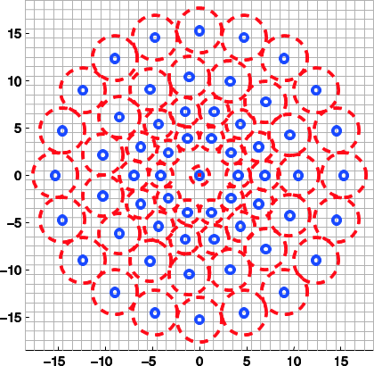
\includegraphics[width=0.48\columnwidth]{2_relworks/brisk}}
    \hfill
    \subfigure[FREAK\cite{alahi_freak:_2012} Sampling Pattern]{\label{fig:markerless_freak}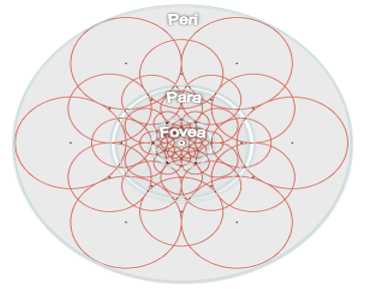
\includegraphics[width=0.48\columnwidth]{2_relworks/freak}}
  \caption{Sampling Patterns of Binary Descriptors}
    \label{fig:markerless_binary_patterns}
\end{figure}


%다음 방법은 matching data structure를 효율적으로 설계하여 nearest neighbor match를 빠르게 수행하도록 하고 있다. 기존의 brute force matching 방법은 query image의 모든 keypoint들을  reference image의 모든 keypoint들과 비교하는 방식으로 가장 속도가 오래 걸리지만, 가장 정확한 nearest neighbor를 검출할 수 있다는 장점이 있다. 이를 개선하기 위하여 다양한 tree 기반의 approximated nearest neighbor 검출 기법들이 사용된다. \cite{beis_shape_1997}에서는 kD tree 기반의 approximation 방법이 제안되었다. 이 방법은 특징의 차원이 비교적 적은 SIFT나 SURF와 같은  vector-value description 방식에서는 좋은 성능을 보여주지만, 최근에 사용되는 binary descriptor에서는 dimension이 높아 성능향상을 기대하기 어렵다는 문제가 있다. LSH\cite{gionis_similarity_1999}와 같은 Hashing 기반의 structure를 이용하여 matching 을 가속화하는 방법도 제안되었다\cite{rublee_orb:_2011}. 이러한 방법은 offline training 단계에서 적절히 특징점들이 고르게 분포하도록 적절한 hash function set을 구성하는 것이 중요하다. 또한, Random Forest\cite{lepetit_keypoint_2006} 또는 Random Fern \cite{ozuysal_fast_2010}은 Binary Description 방식을 Tree 구조 또는 List 구조에 적용하여 matching structure를 구성하였다. 이러한 매칭 방식들은 인식의 속도를 향상시키고, 좀 더 정확한 approximation 값을 얻기 위하여 일반적으로 offline training 단계에서 계산된 descriptor들을 이용하여 추가의 연산을 적용하여 효율적인 matching structure를 생성한다. 하지만, 이러한 방법들을 사용한 추가적인 구조체가 상당히 복잡하고 용량이 크기 때문에 모바일 환경에서 사용하기에 매칭 구조체가 과도하게 무거워진다는 문제점이 존재한다. 또한, detected keypoint의 성질에 대한 고려가 없기 때문에 detected keypoint set이 분류가 어려운 set 일 경우에는 성능 저하가 크게 된다는 한계가 존재한다. 따라서 본 학위논문에서는 이러한 방법을 해결하기 위하여 Keypoint Filtering 기반의 향상된 매칭 방법을 제안한다.

The other researches accelerates nearest neighbor matching with designing an efficient matching data structure. The conventional brute force matching compares all the keypoints of query images with all the keypoints of reference images, so it shows the slowest, but has the advantage of being able to detect the most accurate nearest neighbors. kD tree based approximation method is proposed in \cite{beis_shape_1997}. This method shows good performance in the vector-value descriptor method such as SIFT or SURF with relatively low dimension of features but the improvement of its performance is unlikely to be achieved in the latest binary descriptor with high dimension. A method enabling it to accelerate matching using Hashing based structure in LSH\cite{gionis_similarity_1999} was proposed\cite{rublee_orb:_2011}. As for this method, it is critical to compose appropriate hash function set to distribute the keypoints points evenly in the offline training phase. In addition, 'Random Forest\cite{lepetit_keypoint_2006}' or 'Random Fern\cite{ozuysal_fast_2010}' composed a matching structure by applying a binary description method to the tree structure or list structure. To increase the recognition speed and obtain more accurate approximation values, these matching methods generate efficient matching structure by way of the application of supplementary computation using the descriptors computed in the offline training phase. However, since the supplementary structure that uses this method is complex and large, its the matching structure is too heavy to use in a mobile environment. Moreover, since the properties of the detected keypoints are not taken into consideration, the set for which it is difficult to classify the detected keypoints may lead to performance degradation. To solve this problem, this dissertation proposes a keypoints filtering based matching methods.  

%!TEX root = ../icip_jseo.tex
% -*- root: ../icip_jseo.tex -*-

\section{Keypoint Descriptor Filtering Algorithm}
\label{sec:proposed}

%feature matching 기반의 증강현실 시스템에서는 online process 이전에 reference images들을 오프라인으로 학습(train)하여 비교 대상인 feature database 를 생성하게 된다. 특히 앞의 matching data structure 연구에서 보듯이 온라인 인식의 성능을 높이기 위하여 오프라인 처리에서 다양한 연산을 적용하여 매칭 구조체를 구성함으로써 온라인 인식의 속도나 인식율을 높이기 위한 방법도 제안되고 있다. 
%이러한 기존의 특징점 매칭 방법들은 Feature Detection 알고리즘에서 검출한 특징점을 단순히 모두 학습에 사용하였다. 하지만, 특징점 검출 알고리즘은 Description 알고리즘과 독립적으로 수행되기 때문에 검출(Detect)된 특징점들에 대한 Descriptor가 매칭 성능을 보장할 수 없다는 문제가 있다. 

Feature matching based augmented reality system generates the feature database, the subjects of comparison, by way of the offline training of the reference images before online process. In particular, as shown in the foregoing study of matching data structure, a method that composes a matching structure by applying a various computations to offline process to increase the online recognition speed and recognition rate is proposed. Such established kaypoints matching methods used simply all of the keypoints detected in feature detection module for training. However, since the feature detection algorithm is performed independently from the description algorithm, the descriptor is not able to ensue the matching performance for the detected features. 

%따라서 본 논문에서는 오프라인 학습 과정에서 학습 대상 특징점을 평가하고, 이를 통하여 실시간 인식에 강인한 성능을 제공하는 특징점만을 선정하였다. 이러한 특징점들만을 데이터베이스에 저장함으로써 인식 품질을 유지하면서도 인식 속도를 향상시킬 수 있는 방법을 제안한다.

Thus, in this dissertation, the keypoints of the subjects of training in the offline training process were assessed and only the keypoints providing rigid real-time recognition performance were selected. As a result, a method to increase the recognition speed by saving these features only while maintaining the quality of recognition was proposed. 


\subsection{Definition of Good Keypoins}

%제안하는 방법은 detect된 특징점을 분석하여 인식에 좋은 정도를 측정함으로써 좋은 특징점만을 filtering 한다. 이를 위하여 좋은 특징점을 정의하였다.

The proposed method filters only good keypoints by analyzing the detected keypoints and measuring the degree of the effectiveness of them on recognition, To this effect, good keypoints were defined. 

The conditions of good keypoints for recognition are as follows: 

%첫 번째 인식에 좋은 특징점의 조건은 대상 영상이 다양하게 변화되는 환경에서도 안정적으로 특징점으로 검출되어야 한다는 점이다. 실제 온라인 매칭 과정에서 입력되는 카메라 영상에는 인식하고자 하는 대상 영상이 회전이나 크기, perspective, 노이즈, 조명 등의 다양한 형태의 변환이 적용되어 있다. 인식에 좋은 특징점은 이러한 변환된 영상에서도 안정적으로 특징점이 검출이 됨으로써 Descriptor를 생성할 수 있도록 하는 점이어야 한다.
First, good keypoints need to be stably detected as good points in an environment where targeted images change in various ways. In fact, a wide range of form transformation, such as the rotation, size, perspective, noise and lighting of the targeted images, are applied to the camera images used in the actual matching process. The good keypoints for recognition are detected stably in the converted images, generating descriptors. 

%이러한 안정적 특징점 검출은 Repeatability Score로 측정이 가능하다. Repeatability는 아래 그림과 같이 전체 변환된 영상의 개수 대비 변환된 영상에서 키포인트가 변환되어 존재하는 경우의 비율로 계산된다.
The detection of stable keypoints can be measured by \textit{Repeatability} condition. Repeatability is calculated by the ratio between the total number of converted images and the number of cases where the converted keypoints are existent in the converted images. 


\begin{equation}
p_{repeatability}(p_i) = \frac{n_i^{overlap}}{N}
\end{equation}

% 여기에서 $n_i^{overlap}$는 변환된 영상($T_t(I)$)의 키포인트 집합($K_t'$)에 키포인트($p_i$)가 변환된 점이 존재($T(p_i)\in K_t'$)하는 횟수로 계산되며, $N$은 총 변환된 영상의 개수로 모든 키포인트가 동일한 값을 가지게 된다.

where $n_i^{overlap}$ is calculated by the frequency of the existence of converted keypoint($p_i$) in the set of keypoints($T(p_i)\in K_t'$) of converted images $T_t(I)$; $N$ is the total number of converted images ; and all keypoints have single value. 

%두 번째 인식에 좋은 특징점 집합의 조건은 해당 키포인트가 변화된 영상에서 만들어진 descriptor와의 매치가 실패가 적어야 한다(Similarity)는 점이다.
%이는 해당 특징점의 Sensitivity(True Positive Rate)와 연관이 있다. Reference 영상의 어떤 특징점($p_i$)에 대하여 학습 과정에서 다양하게 변환된 영상($T_t(I)$)에서의 모든 키포인트 집합($K_t'$)의 Descriptor 사이의 매칭을 계산하여 해당 특징점에 대한 Genuine 분포와 Impostor 분포를 계산할 수 있다. 이 때, 해당 키포인트가 변화된 영상에서의 Descriptor와의 매치가 실패가 적기 위해서는, Genuine 분포가 매치 임계 거리(Match Distance Threshold)에서부터 충분히 떨어져 작은 값을 가져야 한다. 이를 위하여 Genuine 분포의 평균을 이용하여 이를 측정하였다. 식 \ref{eq:similarity}에서 보는 것과 같이, Genuine 분포가 작을 수록 좋은 특징점이기 때문에 genuine 분포의 평균을 normalize 하여 1에서 뺌으로써 평가 함수를 계산하였다.

Second, Good keypoints need to be well-matched with identical keypoints even though targeted images change in various ways(\textit{Similarity} condition). With regard to a certain keypoint($p_i$) of reference images, genuine distribution' and imposter distribution' for the corresponding keypoint can be measured by calculating the matching between the descriptors of all the sets of keypoints($p_i$) in images($T_t(I)$) converted in various ways  during the training process. At this time, to reduce the failure in matching the corresponding keypoints and the descriptors in the converted images, the genuine distribution needs to have small value, being far enough away from match distance threshold. To this effect, it was measured using the mean of genuine distribution. As shown in Equation \eqref{eq:similarity}, the keypoints with the decreasing the genuine distribution are better, so the evaluation function was calculated by normalizing the mean of the genuine distribution and subtracting its value from 1.  

\begin{equation} \label{eq:similarity}
p_{similarity}(p_i) = 1 - \frac{\mu_{gen,i} - \min_i \mu_{gen,i}}{\max_i \mu_{gen, i} - \min_i \mu_{gen,i}}
\end{equation}	

%세 번째 조건은 학습된 특징점이 자신과 다른 특징점과는 매치가 이루어지지 않아야 한다(Separability)는 점이다. 이는 각 특징점의 Impostor 분포와 관련이 있다. 다양하게 변화된 영상에서 추출된 특징점 중 자기 자신이 변환된 특징점이 아닌 다른 특징점들과의 매칭 분포를 Impostor 분포라 한다. 어떤 특징점이 자신 이외의 다른 키포인트와 낮은 매칭 성공률을 보여주기 위해서는 Genuine 분포와 Impostor 분포가 잘 구분이 되어야 한다.
%이를 위하여 본 논문에서는 Fisher's Discriminant Ratio\cite{fisher_use_1936}를 이용하였다. 이는 1-dimensional, two class problem에서 sample의 평균과 분산에 의하여 두 클래스 사이의 거리를 측정하는 방식이다. 두 번째 Similarity 조건에 의하여 Genuine 분포가 충분히 작음이 보장이 되었기 때문에 Impostor의 분포가 Genuine 분포에 비하여 충분히 떨어져 있다면 Impostor 분포에 존재하는 특징점들과는 매치가 이루어지지 않음이 보장된다. separability 값 역시 수식 \ref{eq:norm_separability}과 같이 normalize 과정이 필요하다.

Third, the trained keypoints and other keypoints shall not be matched(\textit{Separability}), which is associated with the imposter distribution of each keypoint. Of the keypoints extracted from the images converted in various images, the distribution of the matching with other keypoints rather than the converted keypoints themselves are referred to as imposter distribution. Thus for a specific keypoint to show the low success rate of matching with other keypoints rather than themselves, in is necessary that the genuine distribution and imposter distribution are well classified. To this effect, in this dissertation, \textit{Fisher's Discriminant Ratio\cite{fisher_use_1936}} was used. It measures the distance between two classes by the mean and distribution of sample in 1-dimensional, two class problems. Since the second Similarity condition ensures the genuine distribution is small enough, the nonexistence of the matching with the keypoints in the imposter distribution is ensured if the importer distribution is far enough away compared with the genuine distribution. Separability value also requires the normalization process as shown in equation \eqref{eq:norm_separability}.  


\begin{equation}
FDR(p_i) = \frac{(\mu_{gen,i} - \mu_{imp, i})^2}{\sigma_{gen, i}^2 + \sigma_{imp, i}^2}
\end{equation}
\begin{equation}\label{eq:norm_separability}
p_{separability}(p_i) = \frac{FDR(p_i) - \min_i {FDR(p_i)}}{\max_{i} {s_i}}
\end{equation}	

%이렇게 계산된 세가지 criteria를 이용하여 각 특징점의 score function을 정의할 수 있다. 세 조건은 종속이므로 식 \ref{eq:score_function}와 같이 정의된다.

The score functions of each keypoint can be defined using 3 criteria calculated as above. The 3 conditions are dependent, so can be defined as shown in Equation \eqref{eq:score_function}. 

\begin{equation}\label{eq:score_function}
gf(p_i) = p_{repeatability}(p_i)p_{similarity}(p_i)p_{separability}(p_i)
\end{equation} 



% \subsection{}
%%%%% 시간이 되면 실험 부분을 추가하자 %%%%%





% Below is an example of how to insert images. Delete the ``\vspace'' line,
% uncomment the preceding line ``\centerline...'' and replace ``imageX.ps''
% with a suitable PostScript file name.
% -------------------------------------------------------------------------
% \begin{figure}[htb]

% \begin{minipage}[b]{1.0\linewidth}
%   \centering
%   \centerline{\includegraphics[width=8.5cm]{image1}}
% %  \vspace{2.0cm}
%   \centerline{(a) Result 1}\medskip
% \end{minipage}
% %
% \begin{minipage}[b]{.48\linewidth}
%   \centering
%   \centerline{\includegraphics[width=4.0cm]{image3}}
% %  \vspace{1.5cm}
%   \centerline{(b) Results 3}\medskip
% \end{minipage}
% \hfill
% \begin{minipage}[b]{0.48\linewidth}
%   \centering
%   \centerline{\includegraphics[width=4.0cm]{image4}}
% %  \vspace{1.5cm}
%   \centerline{(c) Result 4}\medskip
% \end{minipage}
% %
% \caption{Example of placing a figure with experimental results.}
% \label{fig:res}
% %
% \end{figure}


% To start a new column (but not a new page) and help balance the last-page
% column length use \vfill\pagebreak.
% -------------------------------------------------------------------------
%\vfill
%\pagebreak


% References should be produced using the bibtex program from suitable
% BiBTeX files (here: strings, refs, manuals). The IEEEbib.bst bibliography
% style file from IEEE produces unsorted bibliography list.
% -------------------------------------------------------------------------
\bibliographystyle{IEEEbib}
% \bibliography{Remote}
\bibliography{reference}

\end{document}
